\documentclass{beamer}

\usetheme{CambridgeUS}
\usecolortheme{beaver}

\title[SSD Energy]{
  Solid State Drive Based Energy Efficient Cloud Storage
}
\author[]{
  Jesus Ramos \and
  Alexis Jefferson \and
  Tiffany Dasilva \and
  Salma Rodriguez \and
  Jorge Cabrera
}
\institute[FIU/VISA]{
  Florida International University \\
  VISA Research Lab \\
  CIS 4911 - Senior Project \\
  Project Mentor: Dr. Ming Zhao
}
\date{December 4, 2012}

\graphicspath{{../images/}}

\begin{document}

\maketitle

\begin{frame}
  \frametitle{Outline}

  \begin{itemize}
    \item Background
    \item Proposed Approach
    \item Implementation
    \item Evaluation
    \item Web Interface
  \end{itemize}

\end{frame}

\section{Background}

\begin{frame}
  \frametitle{Current System}

  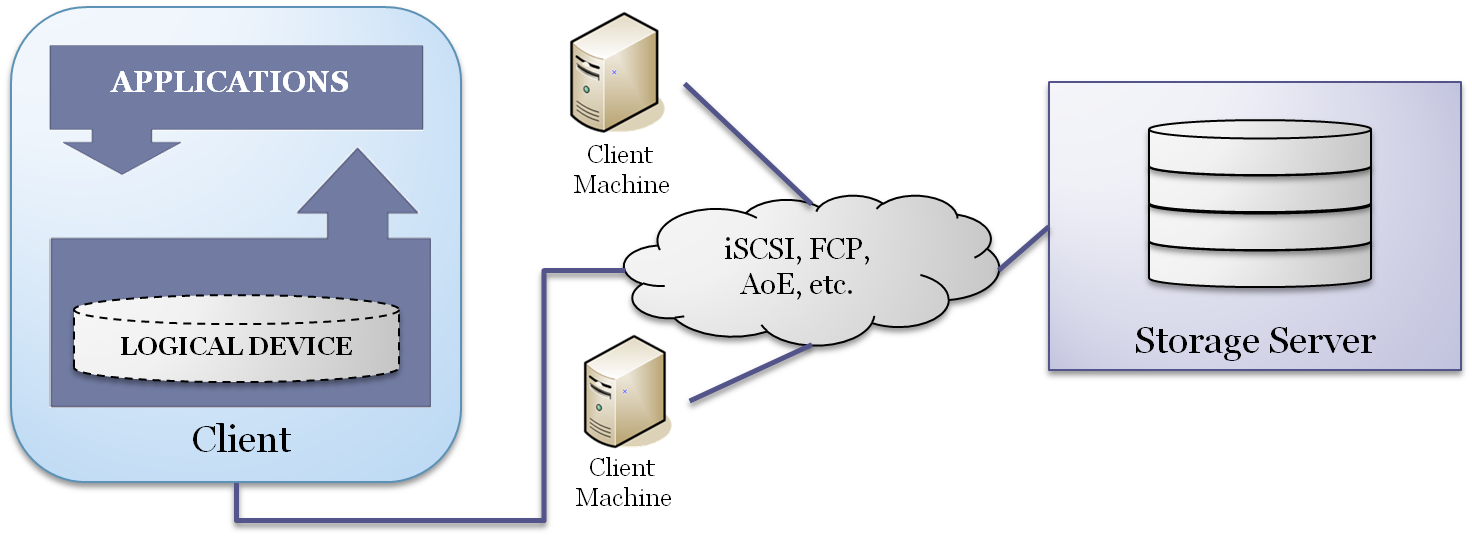
\includegraphics[width=\textwidth,keepaspectratio]{current.png}

\end{frame}

\begin{frame}
  \frametitle{Proposed Approach}

  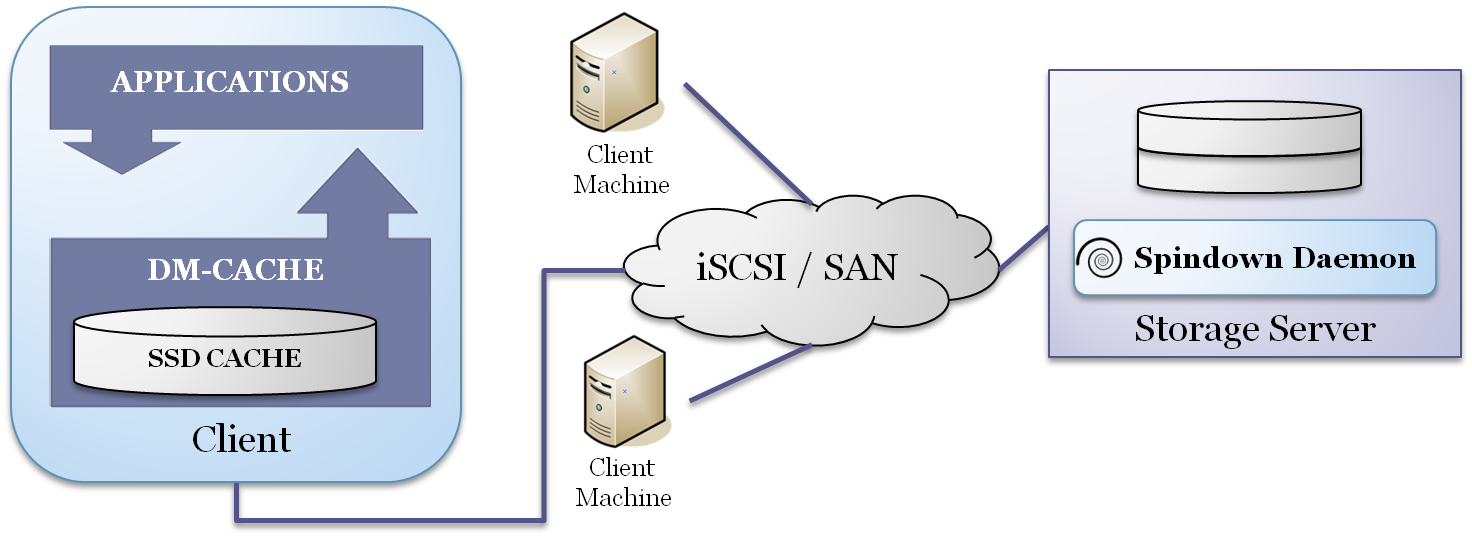
\includegraphics[width=\textwidth,keepaspectratio]{proposed.png}

\end{frame}

\begin{frame}
  \frametitle{Feasibility Study}

  \resizebox{\textwidth}{!}
  {
    \begin{tabular}{|l|l|l|l|}
      \hline
      \bf Disk-State      & \bf Inc. from Inactive & \bf Disk-State      & \bf Inc. from Inactive \\ \hline
      HDD-Inactive:       & +0                     & SSD-Inactive:       & +0                     \\ \hline
      HDD-Idle:           & +4                     & SSD-Idle:           & +0.7                   \\ \hline
      HDD-Active (Read):  & +7.2                   & SSD-Active (Read):  & +3.5                   \\ \hline
      HDD-Active (Write): & +7.6                   & SSD-Active (Write): & +5.1                   \\ \hline
    \end{tabular}
  }

\end{frame}

\section{Implementation}

\begin{frame}
  \frametitle{Cache Management Policy}

  \begin{description}
    \item[LRU (Least Recently Used)] \hfill \\
    Assumes that pages that aren't used for a long time will not be used in the
    near future
    \item[LFU (Least Frequently Used)] \hfill \\
    Pages that are used less frequently should be evicted first
  \end{description}

  Changes to accommodate policies:
  \begin{itemize}
    \item Replace hash table with a radix tree ordered by sectors
    \item Use linked list to manage LRU and LFU schemes
  \end{itemize}

\end{frame}

\begin{frame}
  \frametitle{Dynamic Spin-down Daemon}

  \centering
  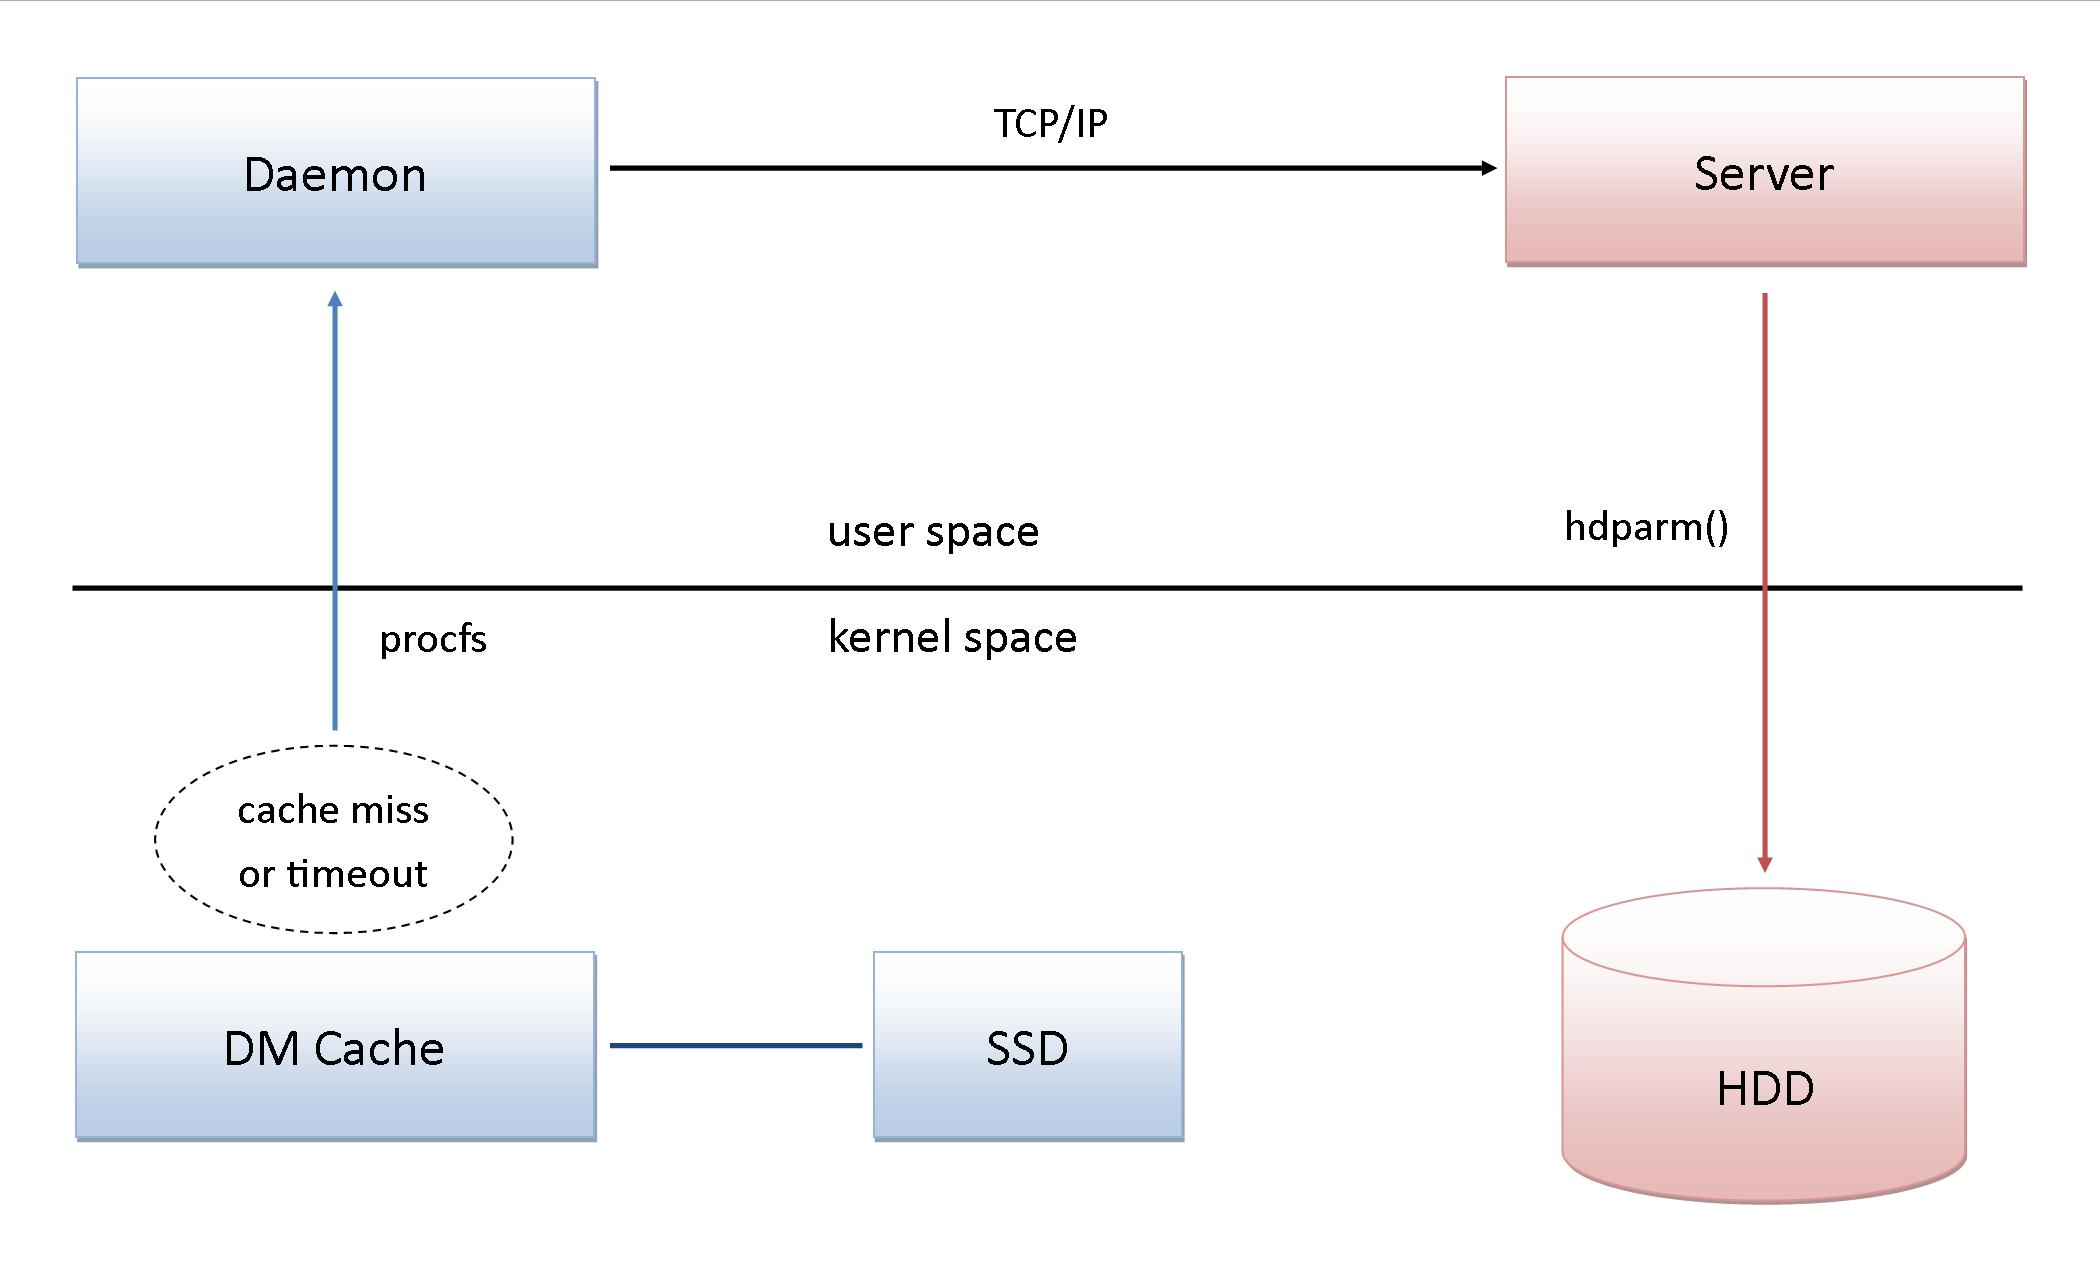
\includegraphics[height=0.8\textheight,keepaspectratio]{daemon.png}

\end{frame}

\section{Evaluation}

\begin{frame}
  \frametitle{IOZone: Micro Benchmarks}

  \begin{columns}
    \begin{column}{0.5\textwidth}
      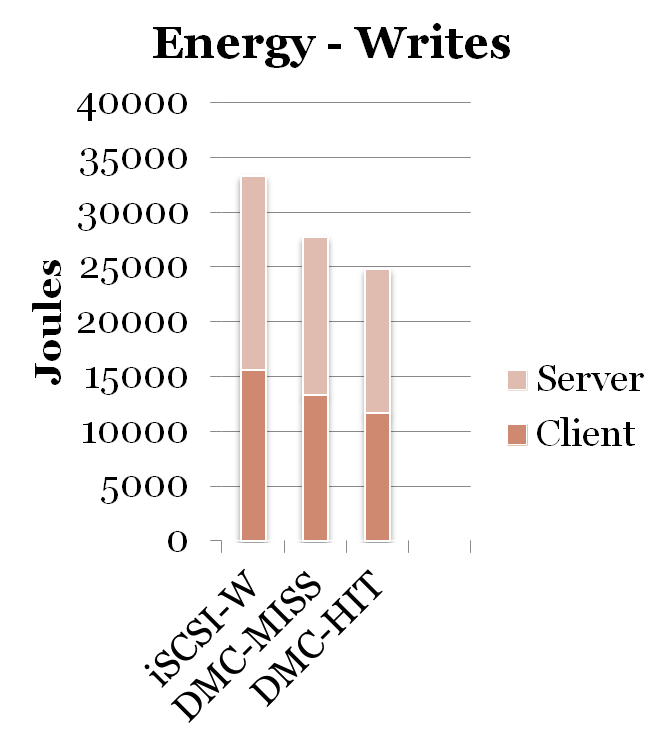
\includegraphics[width=\textwidth]{energy-writes.png}
    \end{column}
    \begin{column}{0.5\textwidth}
      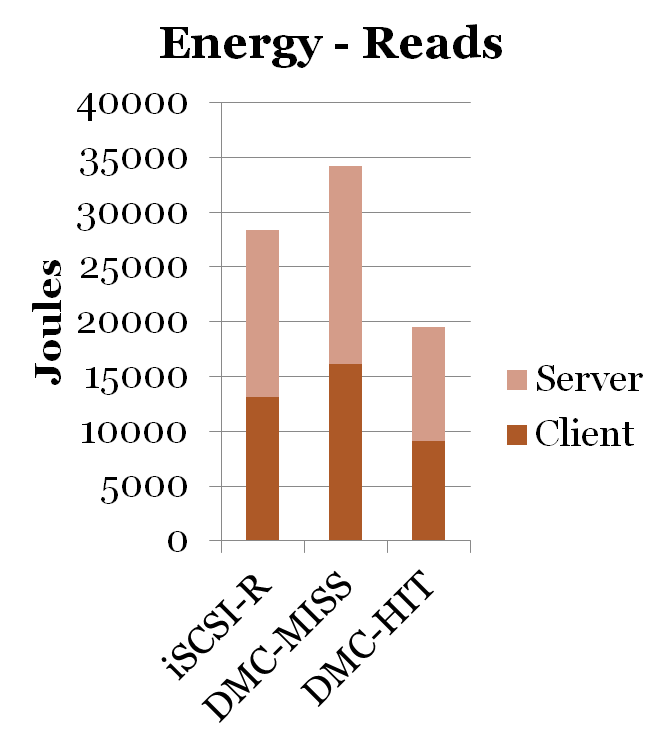
\includegraphics[width=\textwidth]{energy-reads.png}
    \end{column}
  \end{columns}

\end{frame}

\begin{frame}
  \frametitle{Filebench: Synthetic Workload}

  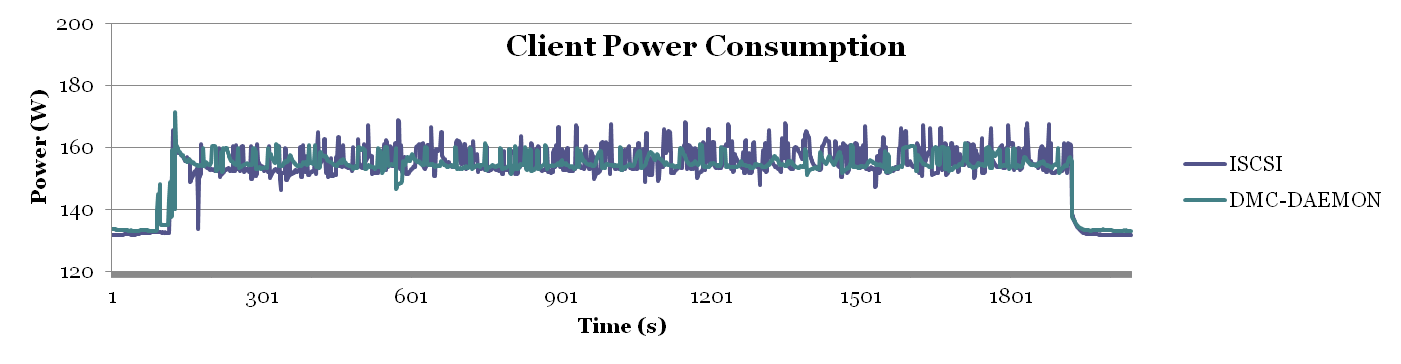
\includegraphics[height=0.4\textheight,width=\textwidth,keepaspectratio]{client-power.png}

  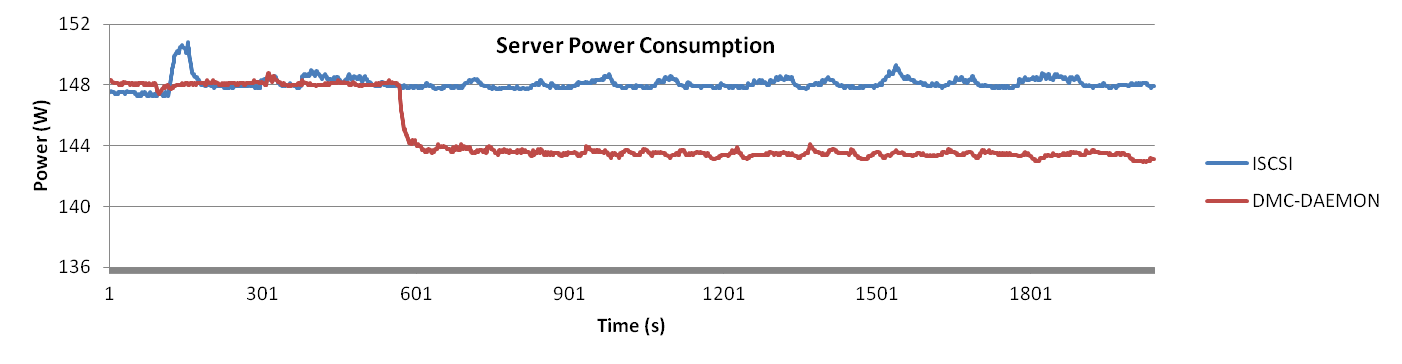
\includegraphics[height=0.4\textheight,width=\textwidth,keepaspectratio]{server-power.png}

\end{frame}

\section{Power Monitoring}

\begin{frame}
  \frametitle{Measuring Power}

  \begin{itemize}
    \item Watts Up? Pro
  \end{itemize}

\end{frame}

\begin{frame}
  \frametitle{Web Application}

  \begin{description}
    \item[Purpose:] display data from measurements
    \item[Important Features:] \hfill \\
    \begin{itemize}
      \item View current power
      \item View past power tests
    \end{itemize}
  \end{description}

\end{frame}

\begin{frame}
  \frametitle{View Past Power}

  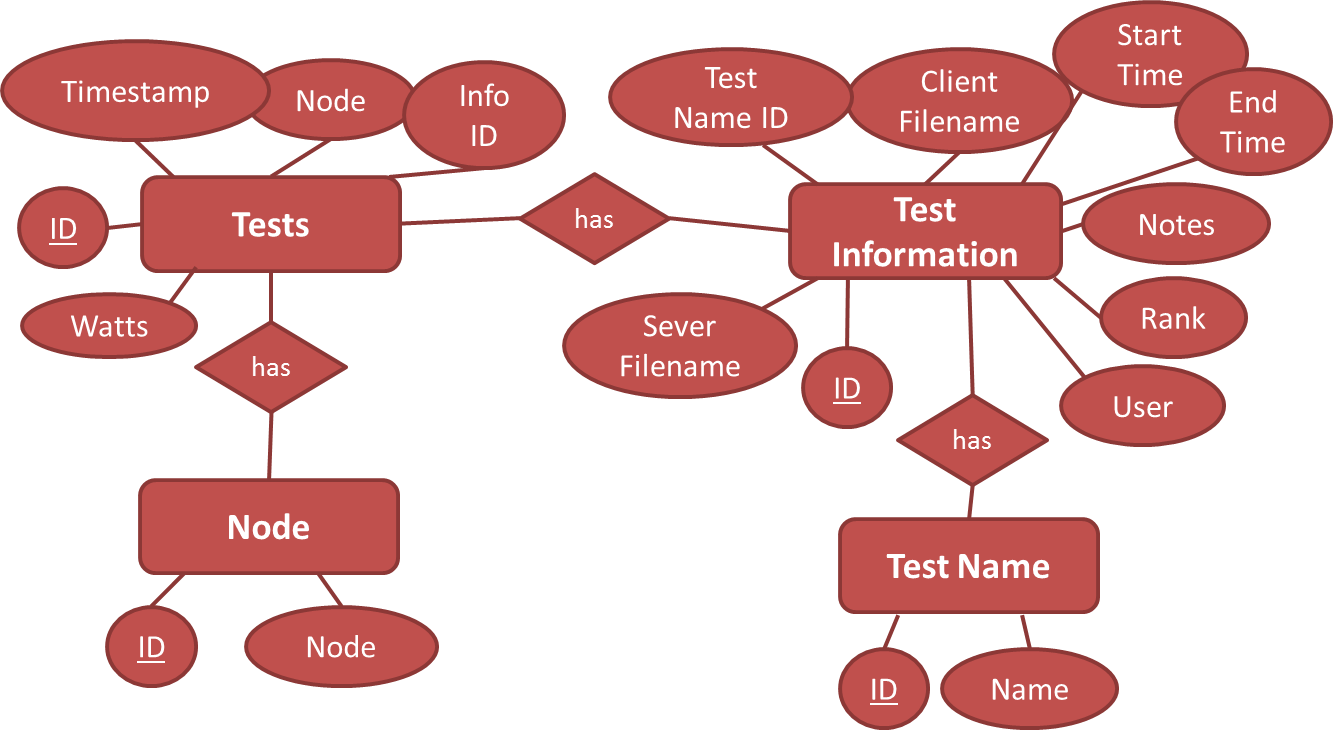
\includegraphics[width=\textwidth,keepaspectratio]{db-diagram.png}

\end{frame}

\begin{frame}
  \frametitle{View Past Power}

  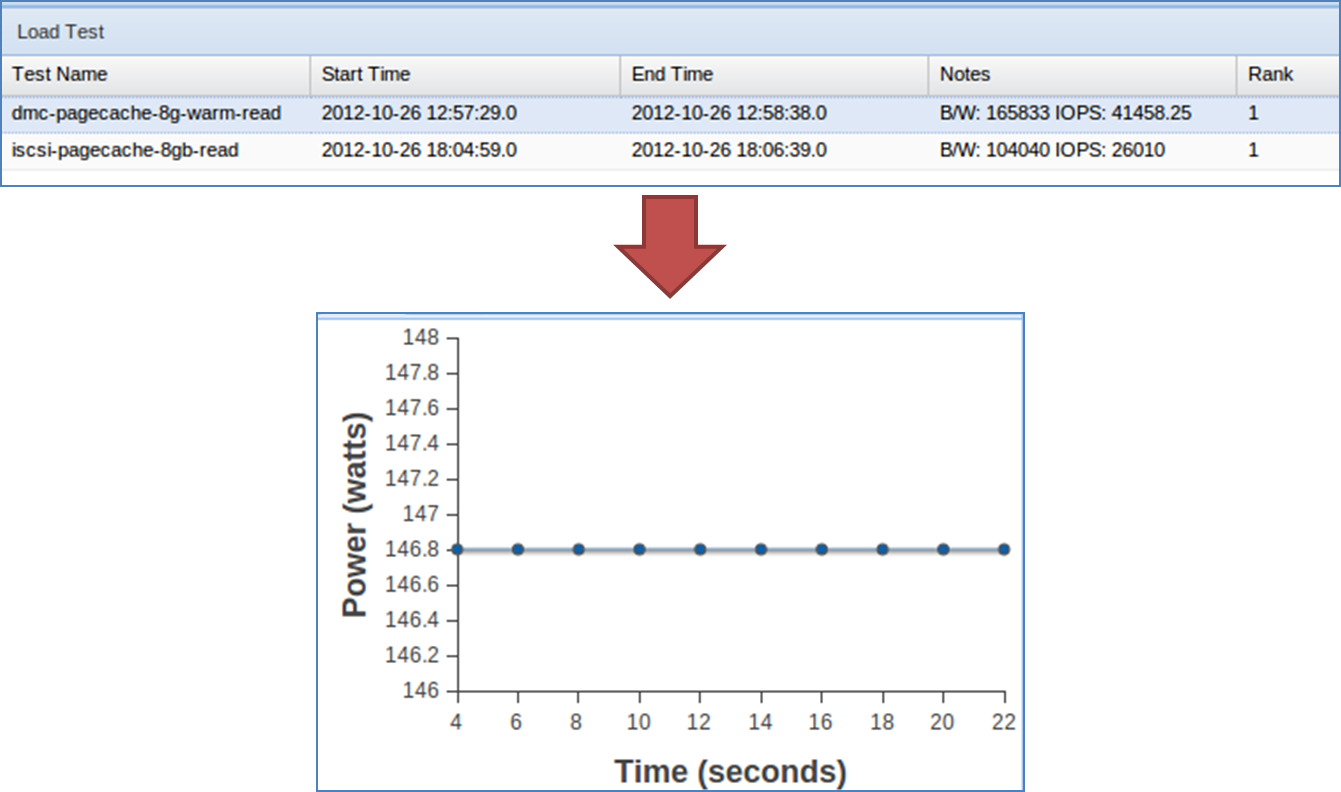
\includegraphics[width=\textwidth,keepaspectratio]{test-to-graph.png}

\end{frame}

\begin{frame}
  \frametitle{View Current Power}

  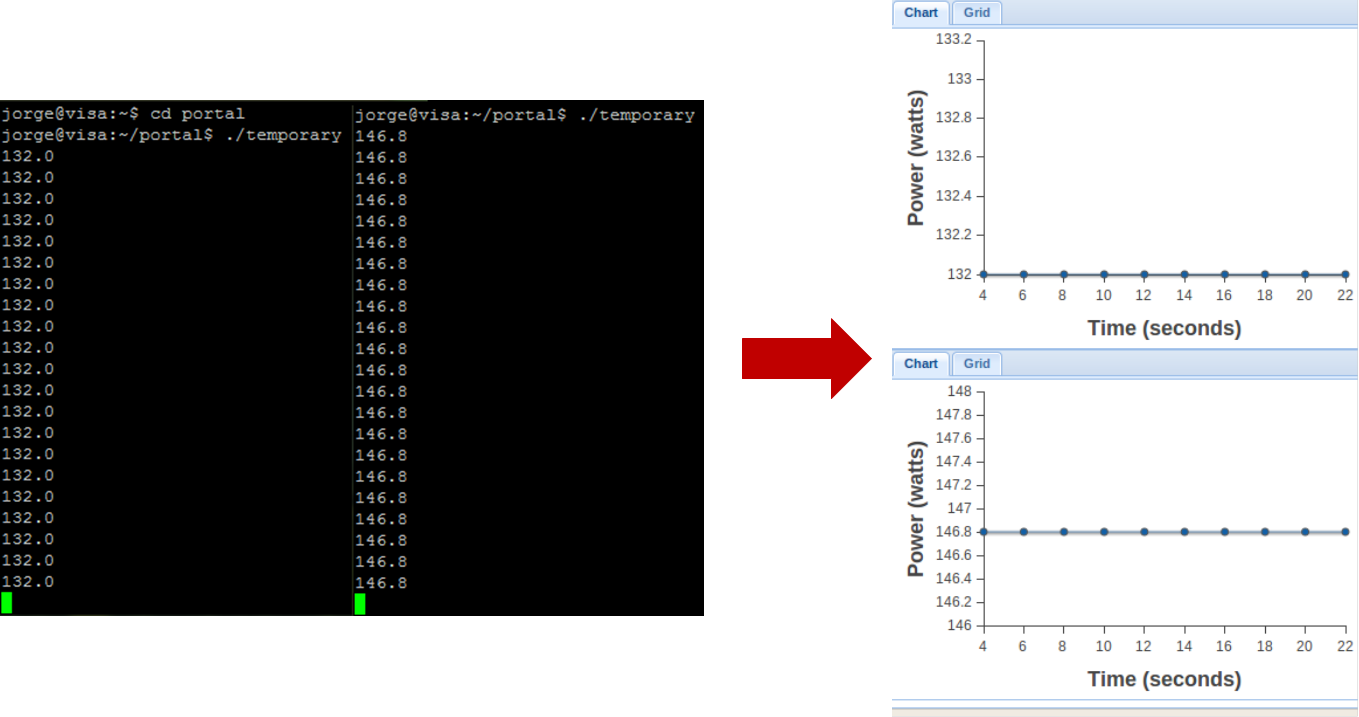
\includegraphics[width=\textwidth,keepaspectratio]{reading-power.png}

\end{frame}

\begin{frame}
  \frametitle{View Current Power}

  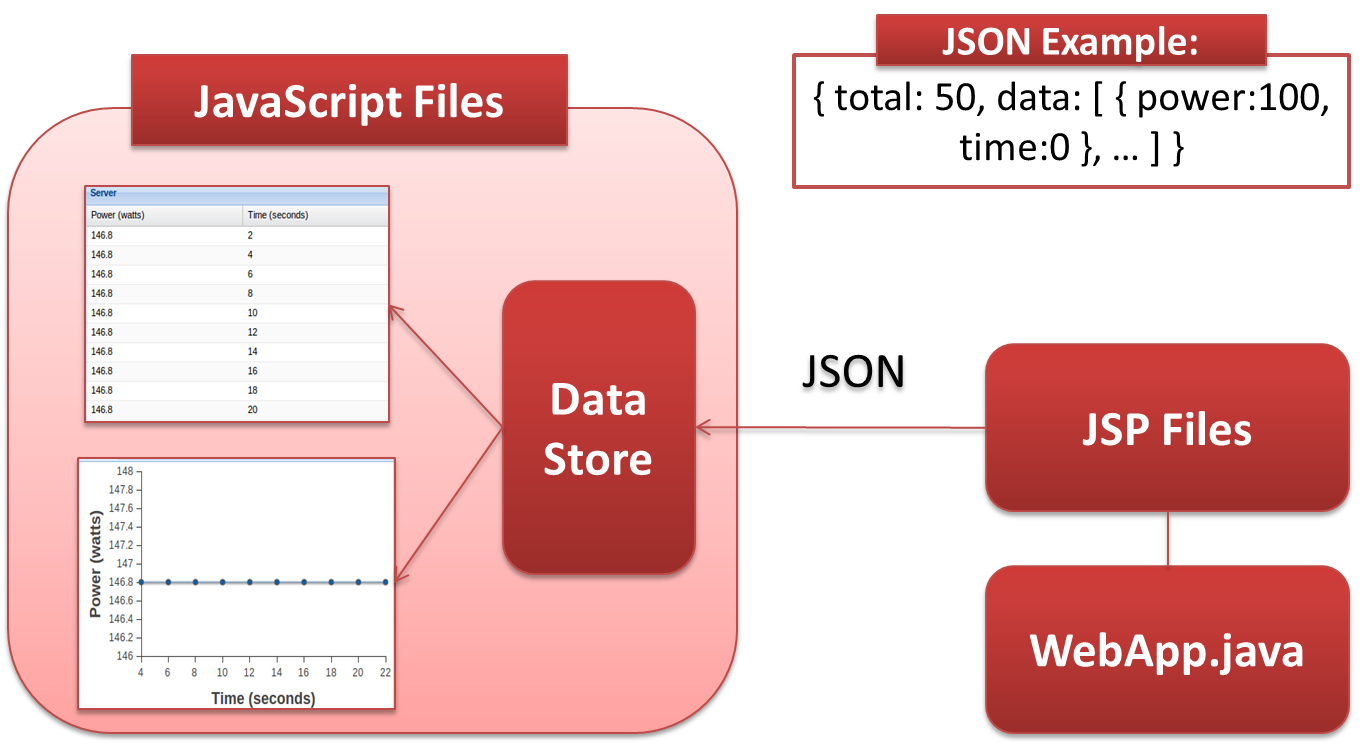
\includegraphics[width=\textwidth,keepaspectratio]{json.png}

\end{frame}

\end{document}